\documentclass{article}

% if you need to pass options to natbib, use, e.g.:
% \PassOptionsToPackage{numbers, compress}{natbib}
% before loading nips_2016
%
% to avoid loading the natbib package, add option nonatbib:
% \usepackage[nonatbib]{nips_2016}

\PassOptionsToPackage{numbers,sort&compress}{natbib}
\usepackage[final]{nips_2016} % produce camera-ready copy

\usepackage[utf8]{inputenc} % allow utf-8 input
\usepackage[T1]{fontenc}    % use 8-bit T1 fonts
\usepackage{hyperref}       % hyperlinks
\usepackage{url}            % simple URL typesetting
\usepackage{booktabs}       % professional-quality tables
\usepackage{amsfonts}       % blackboard math symbols
\usepackage{nicefrac}       % compact symbols for 1/2, etc.
\usepackage{microtype}      % microtypography
\usepackage{graphicx}
\usepackage{comment}
\usepackage{appendix}
\usepackage{float}


\title{Spotify Top Spots: Is There Rhyme or Reason?}

% The \author macro works with any number of authors. There are two
% commands used to separate the names and addresses of multiple
% authors: \And and \AND.
%
% Using \And between authors leaves it to LaTeX to determine where to
% break the lines. Using \AND forces a line break at that point. So,
% if LaTeX puts 3 of 4 authors names on the first line, and the last
% on the second line, try using \AND instead of \And before the third
% author name.

\author{
  S2077483\\
  %% examples of more authors
  \And
  S2595518\\
 \And
  S1977113\\
}

\begin{document}

\maketitle

\begin{abstract}

 This paper seeks to develop a reliable method for predicting if a song will reach the top 10 in the Spotify charts using the song's characteristics and introducing several historical popularity metrics. We found the historical popularity metrics to be key features in improving model accuracy. The best-performing models are concluded to be Random Forest classifier (75.8\% accuracy, 74.2\% F1-score, and 84.3\% ROC AUC) and Extreme Gradient Boosting (78.6\% accuracy, 77.8\% F1-score, and 87.6\% ROC AUC). We then use the Extreme Gradient Boosting model on newly released songs to obtain two potential global top 10 hits. 

 
 
\end{abstract}

\section{Introduction}

Spotify is a widely recognised music streaming platform that offers detailed information on song
characteristics such as danceability, valence, and loudness. Leveraging these features alongside
metrics reflecting the artist’s historical prominence, such as the number of songs previously in top
charts and the average rank of those songs, may play a crucial role in predicting a song’s popularity. These in conjunction can serve as an indicator of the utmost global commercial success. 

 Historical popularity has been explored in the past, with research that utilises low and high-level audio features and the date of the song’s release with deep neural networks \cite{study}. Another study has combined intrinsic song characteristics with social media statistics, selecting a random forest as the best-performing classifier \cite{journal2}. The consideration of prior popularity was also a focal point in a separate research paper, aiming to identify the 20 most significant variables for predicting a song’s popularity. This study revealed that previous popularity significantly influenced the prediction outcome \cite{thesis}. 

This paper seeks to include several historical popularity metrics to improve machine-learning attempts at predicting if a song would reach a top 10 position on the global Spotify charts. 


\begin{comment}

Spotify is a widely recognised music streaming platform, which offers detailed information on song characteristics such as danceability, valence, and loudness. Leveraging these features alongside metrics reflecting the artist's historical prominence, such as the number of songs previously in top charts and the average rank of those songs, may play a crucial role in predicting a song's popularity. Obtaining the forecast for the songs performance can aid in strategic decision making in the music industry. In our research, we aimed to create a machine-learning model to predict if a song would reach a top 10 position on the global charts. This can serve as an indicator of an utmost global commercial success. 

The idea has been explored in the past, with research utilising low and high level audio features and the date of the song's release with deep neural networks \cite{study}. Another study has looked at combining the intrinsic song characteristics with social media statistics, selecting a random forest as the best performing classifier \cite{journal2}. The consideration of prior popularity was also a focal point in a separate research paper, aiming to identify the 20 most significant variables for predicting a song's popularity. This study revealed that previous popularity significantly influenced the prediction outcome \cite{thesis}.
\end{comment}

\section{Data Preprocessing}
The Spotify data used for this paper contains information about a song’s rank on a given day during the span of January 1, 2017, to May 28, 2023. The columns in the dataset that we will focus on include \textit{Rank}, \textit{Title}, and \textit{Date}. There also were seven song characteristics, including \textit{Danceability}, \textit{Energy}, \textit{Loudness}, \textit{Speechiness}, \textit{Accousticness}, \textit{Instrumentalness}, and \textit{Valence}. To prepare this data for data exploration, we begin by dropping the duplicate songs that appear on the same day when multiple artists are in a given song. 


To investigate our interest in the effect of an artist's previous popularity on future popularity, we create four new columns that probe into this idea. \textit{Previous Popularity} refers to whether an artist has ever had a song reach the top ten in the Spotify rankings. \textit{Number of Songs Previous} is the number of songs that an artist has ever shown up in the Spotify top 200 regardless of rank. \textit{Previous Top Rank Avg} is the average top rank an artist’s previous songs.  Lastly, the \textit{Number of Artists} is simply the number of artists that appear in the song. When creating these columns, it was critical to be mindful of the date so an artist's previous popularity and number of songs relate to the date the song first appeared in the charts. This means an artist’s popularity later will not influence their popularity earlier. To accomplish this, we ordered the dataset by date and iterate through each row, keeping track of these variables for each artist to ensure we remained true to what was known at the time. For the case of an artist not having a value for \textit{Previous Top Rank Avg}, we simply encoded them to 201, a value outside of the top 200. Appendix A shows the process of coding these new columns in python jupyter notebook.


	The last set steps included encoding whether a song ever reached the \textit{Top 10} spot, encoded to true or false. We also utilise the standard scaler from the scikit-learn python library to scale the song characteristics. After this, we decided to remove the earliest month in the dataset, as those songs include ones that are at the end of their popularity and would be falsely classified as scoring low on the charts. This is due to insufficient data for these songs before February 1, 2017, causing a song or artist to appear worse than reality, such as if a song did reach the top ten or top one spot before February 1, 2017, but had fallen off below top ten when our dataset begins. It is important to note that we still use the earliest month to create \textit{Previous Popularity}, \textit{Number of Songs Previous}, and \textit{Previous Top Rank Avg}. We only remove the month after. Lastly, we remove all duplicates, keeping only the first occurrence so we only contain one observation for a song created by an artist(s). It is with this dataset we begin our data exploration.


\section{EDA}
There are 693 songs in our records that have reached \textit{Top 10} within the charts and 6808 that have not. With our analysis we aim to uncover the factors that might contribute to a song’s success, explaining why some songs make it to the \textit{Top 10} while others do not. 

We started by exploring the distribution of values for key song characteristics, namely \textit{Danceability}, \textit{Energy}, \textit{Loudness}, \textit{Speechiness}, \textit{Acousticness}, \textit{Instrumentalness}, \textit{Valence}, (as seen in Fig. \ref{fig:dist}). Surprisingly, the visual examination of the figures did not reveal significant differences between the two groups. The disparities in means were minimal, with the highest observed in \textit{Energy} (0.136) and the lowest in \textit{Acousticness} (0.040). These marginal variations suggest that the intrinsic features of songs do not exhibit substantial differences between those that reach \textit{Top 10} status and those that do not.




\begin{figure}[h]
  \centering
  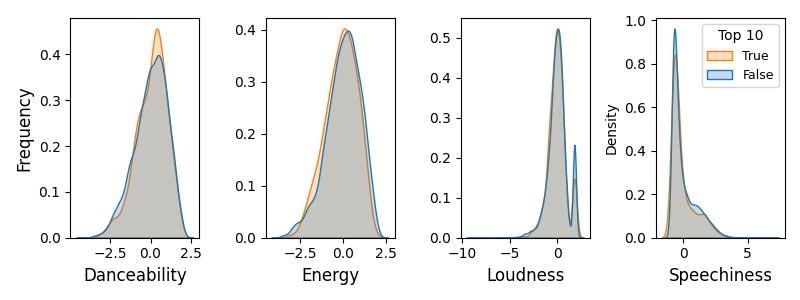
\includegraphics[width=0.8\linewidth]{distplot_chars.png}
  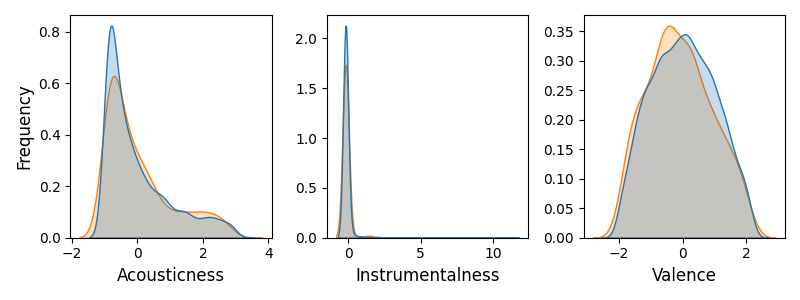
\includegraphics[width=0.8\linewidth]{distplot_chars_rest.png}
  \caption{Distribution of song characteristics for songs in and outside the 'Top 10'.}
  \label{fig:dist}
\end{figure}


To see if an artist's recorded past success contributes to a song’s performance in the charts, we explore the historic popularity metrics, specifically \textit{Previous Popularity}, \textit{Number of Songs Previous}, and \textit{Previous Top Rank Avg}. Overall, 26.0\% of the songs in our dataset have a documented previous popularity, a figure that significantly rises to 49.9\% for songs that have reached the top 10. This suggests a notable relationship between an artist's prior success and their likelihood of producing a chart-topping song.


\begin{figure}[H]
  \centering
  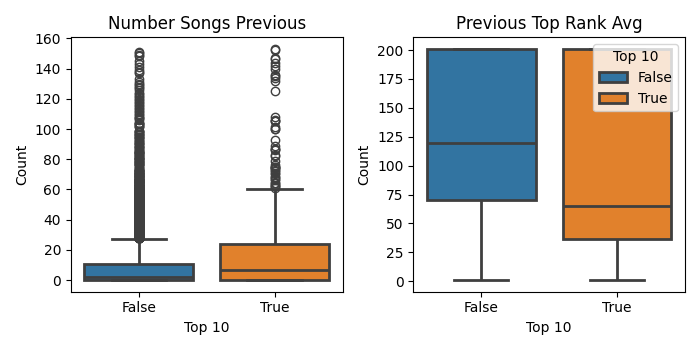
\includegraphics[width=0.8\linewidth]{boxplot.png}
  \caption{Distribution of popularity metrics within and out of the 'Top 10'.}
  \label{fig:box}
\end{figure}

For the latter two metrics, we plotted the distribution for visual inspection. Most artists do not have a high volume of songs that reach the top 200, as indicated by the distribution of counts between the two groups (as depicted in Fig. \ref{fig:box} on the left). This points us in the direction that there are different measures of popularity. The average of the rank of previous songs provides insight into the mean popularity of songs per artist. For songs reaching the top 10, the average position in the chart is notably higher, with a median of 63 versus 119. This implies that songs achieving top positions typically come from artists who have had songs that were consistently high in the top charts. 


\section{Learning Methods}

We followed a systematic methodology to develop a predictive model for determining whether a song will attain a position in the \textit{Top 10} of the global charts. With the cleaned dataset, we defined the features as song characteristics, the number of artists and the historical popularity metrics. The class to be predicted is the \textit{Top 10} column. We applied an 80/20 train-test split with a stratified distribution based on the class label for final model training and evaluation, and a stratified 80/20 train-validation split on the training set for hyperparameter tuning. To address the class imbalance of the \textit{Top 10}, we applied the Synthetic Minority Oversampling Technique (SMOTE) from the imbalanced-learn python library on each one of the sets independently. 

Accuracy is a key metric we used for evaluating the models’ performance. As we have balanced out the distribution of the \textit{Top 10} class, it should give us an overview of a model’s performance. Additionally, we have incorporated the F1 score, which combines precision and recall to ensure that both the false positives and false negatives are considered in the evaluation. As some of the models obtain the class prediction from probabilities, getting the Area Under the Curve of the Receiver Operating Characteristic (ROC AUC) gives us a measure of the model's ability to discriminate between classes across various classification thresholds. 

\subsection{Models}
We employed \textbf{logistic regression} as a simple base classifier, giving us an initial performance to compare against the more complex models. 

The \textbf{K-Nearest Neighbours} (KNN) supervised learning algorithm provides a distance based classification based on the majority class of the k-nearest points in the feature space, in our case for the 5 nearest points obtained by the Euclidean distance \cite{knn}. 

\textbf{Support Vector Machine Classifier} (SVM/SVC) splits the data into 2 classes in a high-dimensional feature space with a hyperplane that maximises the distance between the decision boundary and the nearest data point (support vectors) from both of the classes \cite{svm1}. This margin maximisation contributes to better generalisation on classifying unseen examples \cite{svm}. 

The \textbf{Random Forest Classifier} is an ensemble of individual decision trees, recursively created with a random subset of data and features \cite{inbook}. The variability in the creation of the model increases its generalisation capabilities. To ensure reproducibility, we set a consistent random state. The final prediction is the average of the decision tree voting. The following parameters for tree regularisation where considered in the hyperparameter tuning process:
\begin{itemize}
  \item \texttt{{n\_estimators}}: monitoring the number of trees to be constructed
  \item \texttt{{max\_depth}}: the maximum number of levels per decision tree
  \item \texttt{{min\_samples\_split}}: the minimum number of samples in a node to perform a split
  \item \texttt{{min\_sample\_leaf}}: the minimum number of samples required to be in a childless node \cite{rf_docu}. 
\end{itemize}



A different decision tree ensemble classifier, \textbf{Extreme Gradient Boosting Classifier} (XGBoost), builds decision trees sequentially, with the aim of iterative correction of errors of the previous classifier. The final prediction is formed by combining the predictions made by each tree, each of which is trained on a subset of the data. One distinction between extreme gradient-boosting and Random Forest is that extreme gradient boosting employs a more regularised model, which aids in mitigating the risk of overfitting \cite{xgboost}. The parameters considered and later tuned for the setup of the algorihtm are: 

\begin{itemize}
  \item \texttt{{n\_estimators}}: the number of trees 
  \item \texttt{{max\_depth}}: the maximum height of the trees
  \item \texttt{{learning\_rate}}: step size for adjusting the weights in the boosting process
  \item \texttt{{subsample}}: the ratio of training instance to be resampled before setting up the trees
  \item \texttt{{colsample\_bytree}}: the subsample ratio of columns for each tree \cite{unknown}, \cite{xgboost_docu}.
\end{itemize}



\section{Model Selection}

We first created a base logistic regression model with a maximum number of iterations of 1000 based solely on the numerical song characteristics and excluding the historic popularity metrics. This model produced an accuracy score of 55.2\%, an F1-score of 55.9\%, and an ROC AUC of 59.1\% on the validation set. This base model will be improved upon using the historic popularity metrics we extracted and with the models discussed in the learning methods section. 


\begin{table}[h]
\centering
\caption{Model performance with no parameter adjustment on the validation set}\label{table: 1}
\begin{tabular}{|c|c|c|c|}
\hline
 Model & Accuracy & F1-Score & ROC AUC\\ 
\hline
 Logistic Regression & 66.0\% & 63.2\% & 69.7\% \\
 KNN & 62.3\% & 58.9\% & 65.9\% \\
 SVM & 66.4\% & 62.6\% & 71.0\% \\
 Extreme Gradient Boosting & 83.3\% & 81.6\% & 83.3\% \\
 Random Forest & 77.4\% & 73.0\% & 86.3\% \\
\hline
\end{tabular}
\end{table}

Table 1 displays the different models with the default parameters given by the scikit-learn library on the validation set. These models now include the historic popularity metrics as features along with the song characteristics. The positive impact of the historic popularity metrics is obvious, as the \textbf{Logistic Regression} with them improves its accuracy and F1-score to 66\% and 63.2\%, respectively. It also greatly improved upon the base ROC AUC with a value of 69.7\%. The \textbf{KNN} model performed worse than the logistic regression model but was still better than our base model. It also produced the lowest value for the ROC AUC with 65.9\%, compared to the other models. \textbf{SVM} performs similarly to the logistic regression model but achieves slightly higher accuracy albeit a slightly lower F1-score. The next two models performed the best on the validation set without parameter adjustment. \textbf{Random Forest} achieves a 74.4\% accuracy, a 73\% F1-score, and an ROC AUC value of 86.3\%. In comparison, \textbf{Extreme Gradient Boosting} boasts better accuracy and F1-score of 83.3\% and 81.6\%, respectively, but a lower value for the ROC AUC at 83.3\%. Appendix B details the ROC AUC graph of all the models compared to the base logistic regression model. Having found the two best models, the next step is to tune the parameters in an attempt to improve the models.



\section{Results}
As the random forest and extreme gradient boosting model perform similarly, we hyperparameter tune the models to see if this would reveal any discrepancies in the two models’ performance. The full details of the parameter tuning are shown in Appendix C. For the extreme gradient boosting model, we tuned the model on the validation set, comparing it against its F1-scores and found the best parameterisation of 200 estimators, a max depth of 3, a learning rate of 0.1, a colsample of 0.9, and a subsample of 1. The random forest was similarly tuned on the validation set and compared against its F1-scores. We found this model's best parameterisation to be 200 estimators, a max depth of 10, a minimum sample split of 2, and a minimum sample leaf of 3. Table 2 shows the performance metrics of the tuned models. While both models perform well, the extreme gradient boosting model outperforms the random forest model in all metrics. Notice that the extreme gradient boosting model with parameter tuning receives a worse accuracy and F1-score than its default parameter counterpart. Since the default parameters do not set a tree depth, this can lead to an overfitted model. Thus, while our tuned model appears worse on validation, it is more generalisable to unseen data. With the best parameters found, we recreate the models on the entire training set and test against the unseen test set. The performance of the models on the test set is shown in Table 3. The extreme gradient boosting model on the test set again performs the best compared to the random forest model. Thus, our best model achieves an accuracy of 78.6\%, an F1-score of 77.8\%, and an area under the curve of 87.6\%.  

\begin{table}[h]
\centering
\caption{The tuned models performance on the validation set}\label{table: 2}
\begin{tabular}{|c|c|c|c|}
\hline
Tuned Model & Accuracy & F1-Score & ROC AUC\\ 
\hline
 Extreme Gradient Boosting & 81.9\% & 81.2\% & 90.6\% \\
 Random Forest & 80.3\% & 79.3\% & 88.8\% \\
\hline
\end{tabular}
\end{table}

\begin{table}[h]
\centering
\caption{The tuned models performance on the unseen test set}\label{table: 3}
\begin{tabular}{|c|c|c|c|}
\hline
Tuned Model & Accuracy & F1-Score & ROC AUC\\ 
\hline
 Extreme Gradient Boosting & 78.6\% & 77.8\% & 87.6\% \\
 Random Forest & 75.8\% & 74.2\% & 84.3\% \\
\hline
\end{tabular}
\end{table}

Both the random forest and extreme gradient boosting models greatly utilise the historical popularity metric features, albeit in slightly different ways. The historical popularity metrics account for 50.9\% of the total feature importances. \textit{Previous Popularity} and \textit{Previous Top Rank Avg} are the majority of this, with 21.0\% and 19.4\% respectively. The extreme gradient boosting model places even greater importance on the historical popularity metrics with them accounting for 60.1\% of the total feature importances. However, this model primarily relies on \textit{Previous Popularity}, with a feature importance of 44.7\%. The full list of feature importances for both models are given in Appendix D.


\section{Future Predictions}
The Extreme Gradient Boosting model achieved the best of all three performance metrics of the multitude of models we implemented. With this model in hand, we scoured the web for newly released songs that we thought might reach the top 10 on Spotify. We used songs from popular artists based on the importance of the historical popularity metrics for our models. Importantly, we ensured that the song did not reach inside of the top 20 on the Spotify charts \cite{spotifyCharts}. 

Since our data extent is limited to May 28, 2023, to pull in data for new songs, we incorporated the use of the Spotify web API and spotipy python library. This allowed us to enter in track IDs to pull in the song characteristics of new songs. We also use the same standard scaler, saved as a pickle, to ensure the song characteristics are scaled consistently. However, for the historical popularity metrics, we are restricted to what our cleaned data contained. With this, we built the features for new songs as of late November 2023. The fully constructed data for two songs, Houdini by Dua Lipa and Real Love by Martin Garrix and Lloyiso, are shown in Appendix E.

We predict that Houdini, a song released on November 10, 2023, will reach the top 10 in the Spotify charts. Dua Lipa is a very popular artist, with \textit{Previous Popularity} set to true, 21 \textit{Number Songs Previous}, and a \textit{Previous Song Top Rank Avg} of 41.4. Given her impressive resume, our model has a 76.6\% likelihood that the song, Houdini, would enter the top 10 rankings.

We also predict that Real Love, on September 22, 2023, will also reach the top 10 in the Spotify charts. In contrast to Dua Lipa, these artists are not popular. Based on the data up to May 28, 2023, they have a \textit{Previous Popularity} set to false, 0 \textit{Number Songs Previous}, and a \textit{Previous Song Top Rank Avg} of 201. This shows that the song characteristics still help determine if a song reaches the top 10 in the charts. In this case, the model had a 54.2\% likelihood that the song would enter the top 10 rankings, showing that the historic popularity metrics make a good song more likely to enter the top 10, but it is not an all-encompassing feature.



\section{Conclusion}
In conclusion, the previous popularity metrics proved to be an important part of the prediction of the song reaching Top 10 in the charts, improving our model's classification abilities. Our best-performing model is Extreme Gradient Boosting with the tuned parameters, achieving 87.6\% ROC AUC. 

The model can also identify songs that can reach the top 10 in the Spotify rankings without requiring "good" historical popularity scores. This is incredibly important as an ineffective model would consider all songs from a popular artist to be in the top 10 rankings or all songs from a nonpopular artist to never reach the top 10, which we know does not reflect reality. Thus, our model functions well in its intent, separating good songs capable of top-10 status from those that are not. The historical popularity metrics are some of the most important features in the random forest and extreme gradient boosting models, greatly increasing the performance and confidence in our model's decisions.

One limitation to our approach for checking artist's popularity is that the songs with multiple artists it was obtained for the collaboration. A potential way to improve this would be to establish the individual popularities and devise methods to consolidate them into one. 

For the artists with no previous record in the charts, we assigned their existing rank average to be 201. However, it's worth noting that this approach may be somewhat misleading, as it implies a position just below the top 200 charts, which may not accurately reflect the actual scenario. 


\bibliography{refs.bib}
\bibliographystyle{plain}




\section*{Appendices}
\begin{appendices}
\section{Data Processing Code}
The creation of the historical popularity metrics required diligent and careful manipulation of the data in order to be in respect to time. The two figures below detail our process to create these new columns. Assume that the dataframe \textit{df} has already dropped the duplicate rows, sorted \textit{Date} in nondescending order, and created \textit{Highest Rank} by taking the minimum of \textit{Rank} as grouped by \textit{Atists} and \textit{Title}.

To create \textit{Previous Popularity} and \textit{Number Songs Previous} we iterate through the dataframe row by row, beginning at the earliest date in the dataset, January 1, 2017. Two dictionaries help keep track of these features. \texttt{artist\_top\_ten} holds the artist as a key, and a value of either True or False depending on if the artist has a song that has previously reached the top 10 in the charts. It also verifies that if setting the \texttt{artist\_top\_ten} to true, the song must already have been in the dataset. This helps fix the edge case where a song enters the top 10 on the first day of its arrival in the charts. This way, we keep it limited to \textit{previous} popularity.

The second dictionary \texttt{artist\_songs\_previous} holds the artist as the key, and a growing list of songs as the value. Here, we set \textit{Number Songs Previous} to the length of the list before adding in the current row. 

\begin{figure}[H]
  \centering
  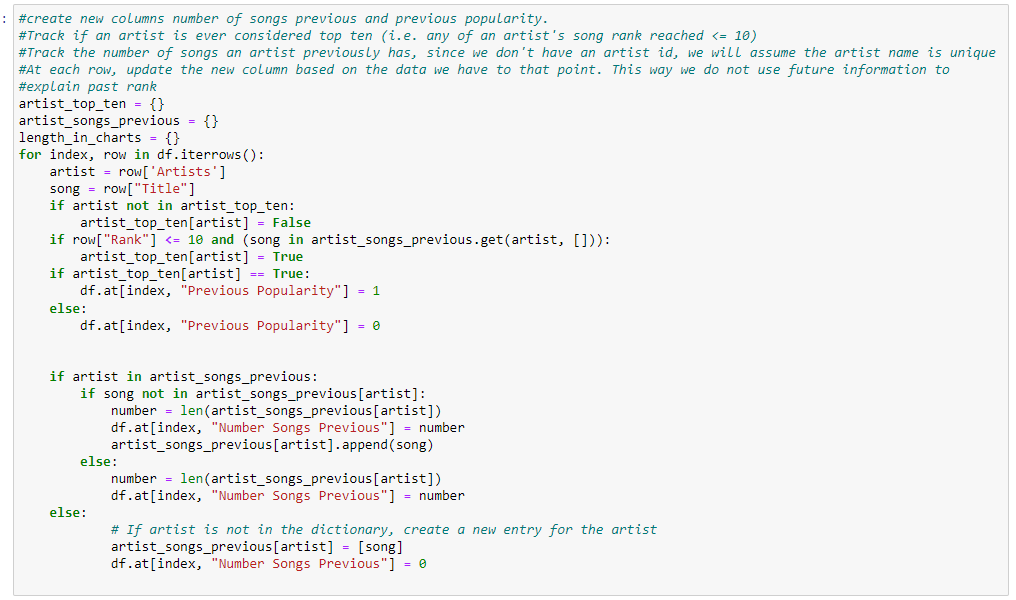
\includegraphics[width=0.9\linewidth]{previousPopCode.png}
  \caption{Creation of \textit{Previous Popularity} and \textit{Number Songs Previous}.}
  \label{fig:dist}
\end{figure}

This last block of code drops the duplicate songs, keeping only the first. We create the standardised song characteristics using standard scaler and save it as a pickle. From there, we calculate \textit{Previous Top Rank Avg} using a dictionary. The artist is the key with the list of each song's highest rank as the value. We initalise the mean to 201, and then calulate the mean of the list before appending in the current song's highest rank.

Lastly, we dropped the first month in the dataset, giving us our cleaned dataset.

\begin{figure}[H]
  \centering
  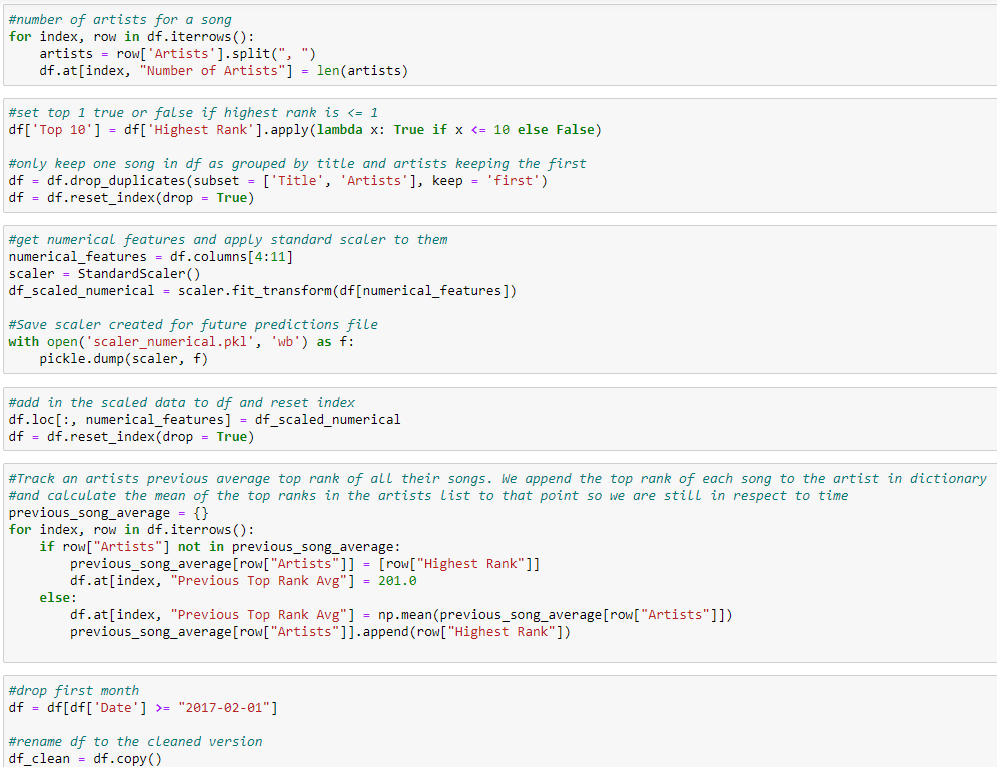
\includegraphics[width=0.9\linewidth]{topRankAvgCode.png}
  \caption{Creation of \textit{Previous Top Rank Avg} and standardising of the song characteristics.}
  \label{fig:dist}
\end{figure}




\section{Models ROC AUC}
\begin{figure}[H]
  \centering
  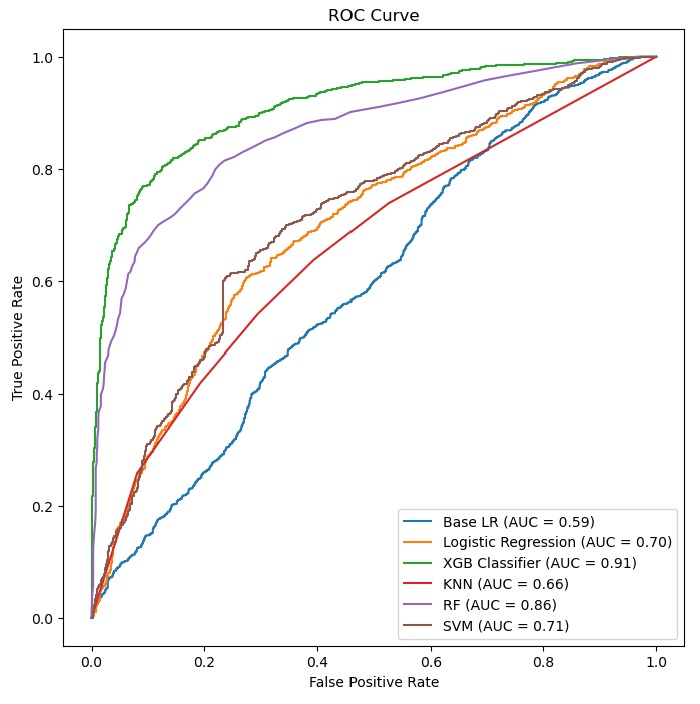
\includegraphics[width=0.8\linewidth]{rocCurve.jpg}
  \caption{ROC AUC Graph for Model Selection in comparison to the Base Logistic Regression model. All models were tested on the validation set.}
  \label{fig:dist}
\end{figure}


\section{Hyperparameter tuning details}
This details the parameters tested while hyperparameter tuning the random forest and extreme gradient-boosting model. This was performed on the validation set and saving the parameters with the best F1-score.
\subsection{Random Forest Hyperparameter Tuning}
\begin{itemize}
    \item Number of estimators: [100, 200, 300]
    \item Maximum Depth: [1, 2, 5, 10]
    \item Minimum Samples Split Values: [2, 4, 6]
    \item Minimum Samples Leaf Values: [1, 2, 3]
\end{itemize}

\subsection{Extreme Gradient Boosting Hyperparameter Tuning}
\begin{itemize}
    \item Number of estimators: [100, 200, 300]
    \item Learning Rate: [0.01, 0.1, 0.2]
    \item Maximum Depth: [3, 5, 10]
    \item Subsample: [0.8, 0.9, 1.0]
    \item Colsample by Tree: [0.8, 0.9, 1.0]
\end{itemize}


\section{Models feature importance}
\begin{figure}[h]
  \centering
  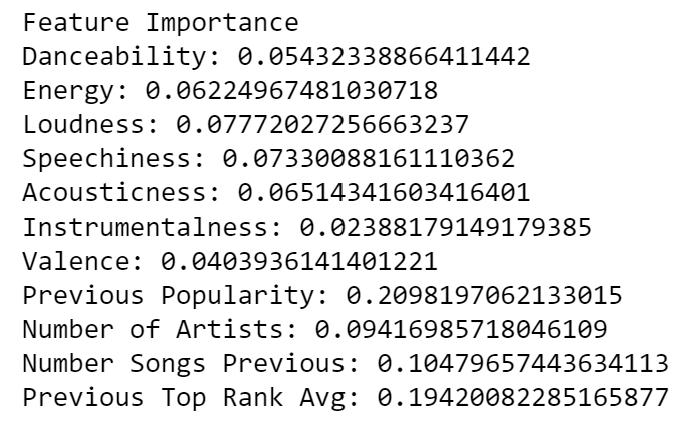
\includegraphics[width=0.5\linewidth]{RFFeatureImp.png}
  \caption{Feature Importances for the hyperparameter tuned Random Forest model on the test set.}
  \label{fig:dist}
\end{figure}


\begin{figure}[h]
  \centering
  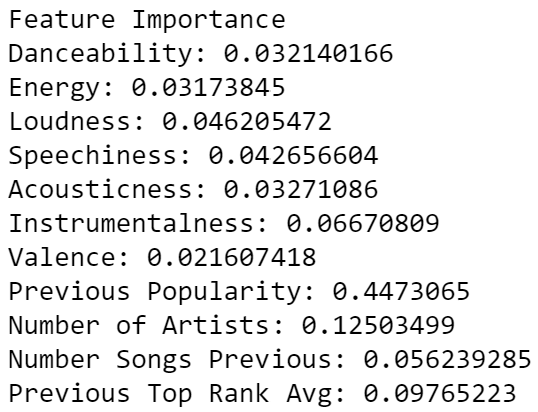
\includegraphics[width=0.5\linewidth]{xgboostFeatImp.png}
  \caption{Feature Importances for the hyperparameter tuned Extreme Gradient Boosting model on the test set.}
  \label{fig:dist}
\end{figure}


\section{Future Prediction Song Features}
\begin{table}[H]
\small
\centering
\caption{Features of the newly released songs for future predictions using the Spotify API for the song characteristics.}\label{table: 4}
\begin{tabular}{|c|c|c|c|c|c|c|c|c|}
\hline
 Song Name & Artist & Danceability & Energy & Loudness & Speechiness \\ 
\hline
 Real Love & Martin Garrix, Lloysio & -0.311 & 0.702 & 0.416 & -0.342 \\
 Houdini & Dua Lipa & 0.595 & 1.021 & 0.780 & -0.141 \\
\hline
\end{tabular}
\end{table}



\begin{table}[H]
\small
\centering
\caption{Features of the newly released songs for future predictions using the Spotify API for the song characteristics.}\label{table: 4}
\begin{tabular}{|c|c|c|c|c|c|c|c|c|}
\hline
 Song Name & Artist & Acousticness & Instrumentalness & Valence  \\ 
\hline
 Real Love & Martin Garrix, Lloysio & -0.758 & -0.375 & -1.042 \\
 Houdini & Dua Lipa & -0.845 & 0.021 & 1.876 \\
\hline
\end{tabular}
\end{table}


\begin{table}[H]
\small
\centering
\caption{Features of the newly released songs for future predictions using our cleaned dataset for \textit{Previous Popularity} and \textit{Number Songs Previous}.}\label{table: 4}
\begin{tabular}{|c|c|c|c|}
\hline
 Song Name & Artist & Previous Popularity & Number Songs Previous \\ 
\hline
 Real Love & Martin Garrix, Lloysio & 0.0 & 0.0  \\
 Houdini & Dua Lipa & 1.0 & 21.0  \\
\hline
\end{tabular}
\end{table}

\begin{table}[H]
\small
\centering
\caption{Features of the newly released songs for future predictions using our cleaned dataset for \textit{Previous Top Rank Avg} and \textit{Number of Artists}.}\label{table: 4}
\begin{tabular}{|c|c|c|c|}
\hline
 Song Name & Artist & Previous Top Rank Avg & Number of Artists  \\ 
\hline
 Real Love & Martin Garrix, Lloysio & 201.0 & 2 \\
 Houdini & Dua Lipa & 41.4 & 1 \\
\hline
\end{tabular}
\end{table}

\end{appendices}

\section{Individual Contributions}


\textbf{S2077483:}

\textbf{Data exploration}: 
\begin{itemize}
    \item performed EDA on the dataset, raw and cleaned
    \item applied the cleaning process
    \item data preprocessing for model predictions, synthetic sampling to balance out the class distribution (SMOTE), split up for the training/val/test sets 
\end{itemize}

\textbf{Model development}: Worked on developing the final models with a focus on the non-tree dependent classifiers: Logistic Regression, SVM, KNN. Explored the potential of applying neural networks for this problem, obtaining preliminary results for a Multilayer Perceptron model. However, we have decided against including this in the report. Developed the workflow for the best model selection, with the utilisation of a baseline model. 
\begin{itemize}
    \item set up for the models
    \item parameter tuning
    \item obtaining the models performance for the 
    \item visualisation of model's performance, ROC AUC curve
\end{itemize}

\textbf{Report}: Wrote sections for the Abstract, Introduction, EDA, Learning Methods and Conclusions. 


\textbf{S2595518:} 
\begin{itemize}
    \item I researched our topic and helped to write the reflective abstract and introduction parts. Moreover, I did research about past written papers and observations and summarized them in the introduction section.
    \item  In addition to this, I have explained some of the models and parameters we used during the project in the Learning Methods section. 
    \item  Lastly, I have helped with the future predictions part by finding famous artists' songs that were released after May 28, 2023, by using Spotify history charts. With the help of our model, we made predictions about whether the songs would be top 10 in the charts.
\end{itemize}

\textbf{S1977113:}

\textbf{EDA/Data Preprocessing/Future Predictions}:
\begin{itemize}
    \item EDA on raw dataset
    \item created columns for previous popularity, number of songs previous, previous top rank avg, number of artists, and top 10.
    \item scaled song characteristics
    \item data cleaning
    \item set up Spotify API, pulled song characteristics of new songs.
    \item created script to generate the dataset for new songs to feed into the model for future predictions based on the song characteristics given by Spotify API and historical popularity metrics from the cleaned dataset.
\end{itemize}

\textbf{Model Development}: worked on the development of random forest, XGBoost, logistic regression, and Base logistic regression models. Hyperparameter tuned the xgboost model. graphed developed models on roc auc curve

\textbf{Report}: wrote sections for Data Processing, Model Selection, Results, Future Predictions and the respective appendicies. Contributed elements of the conclusion. 





\subsection{AI use declaration}

We have used both Github Copilot and ChatGPT for the production of parts of the code, with the usage clearly stated in the code. 
used for: annotating count plots in the EDA (not used included in the report), quick generation of song characteristics from Spotify API to be joined with the cleaned dataset. 
\end{document}

%%% Local Variables:
%%% mode: latex
%%% TeX-master: t
%%% End:
